\documentclass[]{article}

\usepackage[top=1.5cm, bottom=1.5cm, left=3cm, right=3cm]{geometry}

\usepackage{graphics}

\usepackage{graphicx}

\begin{document}
	
\begin{figure}[h]
\centering
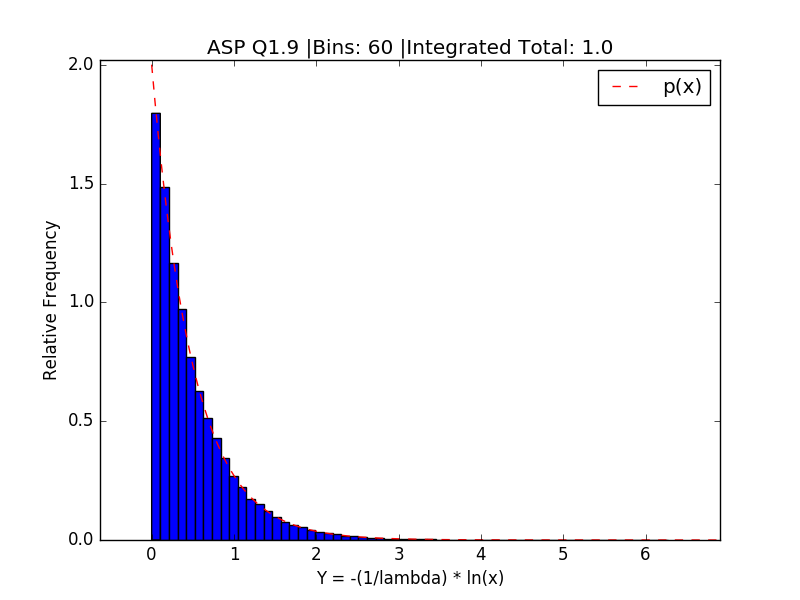
\includegraphics[width=0.6\linewidth]{one_nine}
\end{figure}


\begin{figure}[h]
	\label{fig:parabola_1a}
	\centering
	\begin{minipage}[h]{0.45\linewidth}
		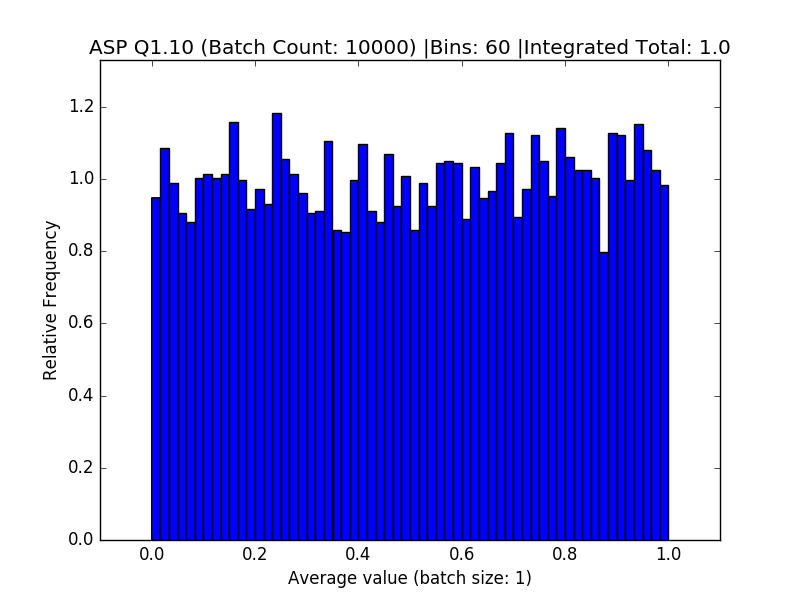
\includegraphics[width=1\linewidth]{one_ten_one}
	\end{minipage}
	\quad
	\begin{minipage}[h]{0.45\linewidth}
		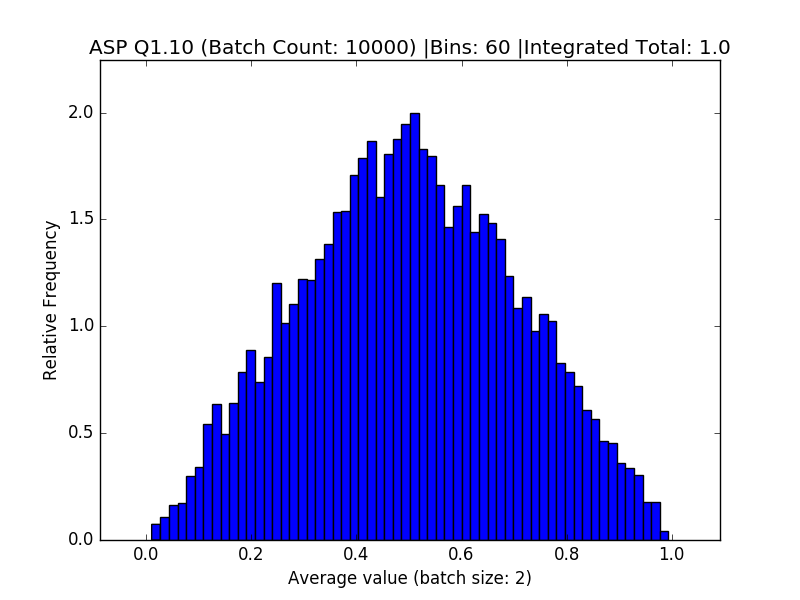
\includegraphics[width=1\linewidth]{one_ten_two}
	\end{minipage}
\end{figure}
\begin{figure}[h]
	\centering
	\begin{minipage}[h]{0.45\linewidth}
		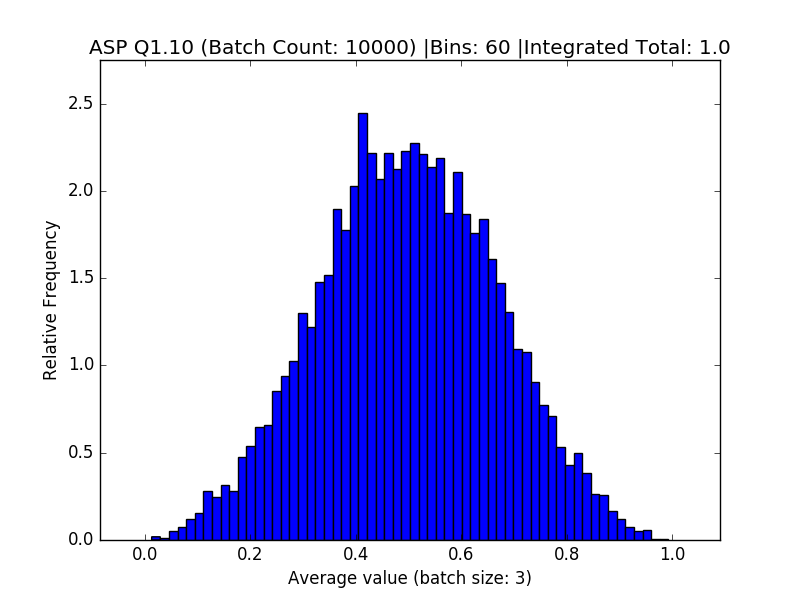
\includegraphics[width=1\linewidth]{one_ten_three}
	\end{minipage}
	\quad
	\begin{minipage}[h]{0.45\linewidth}
		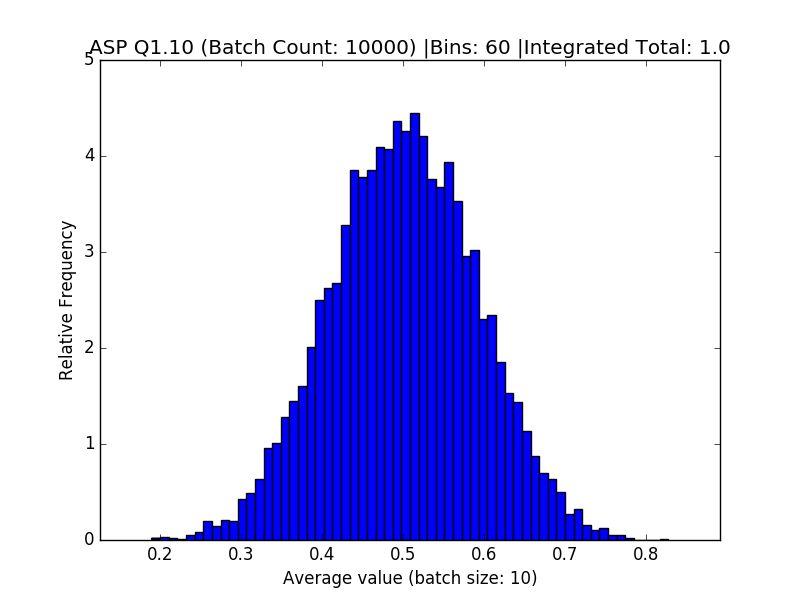
\includegraphics[width=1\linewidth]{one_ten_ten}
	\end{minipage}
\end{figure}


\end{document}
